\documentclass[10pt]{article}
\usepackage{../../local}
\urlstyle{same}

\newcommand{\classcode}{Physics 112}
\newcommand{\classname}{Introduction to Thermodynamics and Statistical Mechanics}
\renewcommand{\maketitle}{%
\hrule height4pt
\large{Eric Du \hfill \classcode}
\newline
\large{HW 08} \large{\hfill \classname \hfill} \large{\today}
\hrule height4pt \vskip .7em
\small{Header styling inspired by Berkeley's CS 70: \url{https://www.eecs70.org/}}
\normalsize
}
\linespread{1.1}
\begin{document}
	\maketitle
	\section*{Collaborators}
	I worked with \textbf{Andrew Binder, David LaRoche, Karen Makino, Nathan Song} and \textbf{Adarsh Iyer} on this 
	assignment.
	\section*{Problem 1}

	Cold Interstellar molecular clouds often contain the molecule cyanogen (CN) whose first rotational 
	excited states have an energy of \(\epsilon_0 = 4.7 \times 10^{-4}\) eV above the ground state. 
	In 1941, studies revealed that starlight passing through these molecular clouds showed that 29 percent 
	of the CN molecules are in the first excited rotational state. To account for this data, astronomers 
	suggested that the CN molecules might be in thermal equilibrium with a reservoir at a 
	well defined temperature.

	 \begin{enumerate}[label=\alph*)]
		\item The energy of the rotational state with angular momentum \(j (j = 0, 1, 2, \dots)\) is 
			given by \(\epsilon(j) = \epsilon_0 j(j+1) / 2\), and the degeneracy of the level (i.e. 
			number of states with the same energy) is \(\Omega(j) = 2j+1\). Note that 
			the ground state has \(j = 0\). Find an expression for the temperature of the thermal reservoir
			as a function of the fraction \(x\) of the excited CN molecules. For simplicity, neglect 
			occupation of states with \(j > 1\) 

			\begin{solution}
				First, we can calculate \( \mean E \) in terms of the fraction of ionized energy:
				\[
					\mean{E} = \epsilon_0 x
				\] 
				Calculating the partition function:
				\[
					Z = 1 + 3e^{-\epsilon_0 / k_BT}
				\] 
				Then, we can come up with an expression for the probability of being in the first excited state:
				\[
					P(j = 1) =  \frac{3e^{-\epsilon_0 /k_B T}}{1 + 3e^{-\epsilon_0/k_BT}} = \frac{3}{e^{\epsilon_0 \beta} + 3}
				\]
				Then, since \( x \) is the fraction of excited molecules, this is also equal to the probability 
				of the particles being in the excited state, so we can just set this equal to \( x \). Then, 
				we can simplify:
				\[
				\frac{3}{e^{\epsilon_0 \beta} + 3} = x \implies T = \frac{\epsilon_0}{k_B \ln \left( \frac{3}{x} - 3 \right) }
				\] 
			\end{solution}
		\item Evaluate your answer from part (a) to find the temperature corresponding to the 
			observed excited fraction. What do you think is the origin of the thermal 
			radiation with which the CN molecule is in equilibrium?

			\begin{solution}
				Plugging \( x = 0.29 \) into this equation gives a temperature \( T = \text{2.73 K} \). The 
				reason it has this temperature is likely due to the residual heat of the CMB, which is responsible
				for the ``ambient temperature'' of the universe.  
			\end{solution}
		\item Justify the assumption made in (a), that all the molecules are either in the ground or first 
			excited state (Hint: Using your temperature from part (b), compute the fraction of molecules 
			that will be in the second excited state.) 

			\begin{solution}
				To calculate this quantity, we first need to modify the partition function to admit the 
				second energy level:
				\[
				Z = 1 + 3e^{-\epsilon_0 \beta} + 5e^{-3\epsilon_0 \beta}
				\] 
				Therefore, the probability of being in the second state is:
				\[
				P(j = 2) = \frac{5e^{-3\epsilon_0 \beta}}{Z} = 0.0087
				\] 
				This means that the probability is \( 0.8\% \), so we are justified in our assumption that 
				\( j > 1 \) states aren't occupied. 
			\end{solution}
	\end{enumerate}
	\pagebreak
	\section*{Schroeder 7.5}
	Consider a system consisting of a single impurity atom/ion in a semiconductor. Suppose that the impurity 
	atom has one ``extra'' electron compared to the neighboring atoms, as would a phosphorous atom occupying 
	a lattice site in a silicon crystal. The extra electron is then easily removed, leaving behind 
	a positively charged ion. The ionized electron is called a \textbf{conduction electron},
	because it is free to move through the material; the impurity atom is called a \textbf{donor}, because it 
	can ``donate'' a conduction electron. This system is analogous to the hydrogen atom considered in the
	previous two problems except that the ionization energy is much less, mainly due to the 
	screening of the ionic charge by the dielectric behavior of the medium. 
	\begin{enumerate}[label=\alph*)]
		\item Write down the formula for the probability of a single donor atom being ionized. Do not 
			neglect the fact that the electron, if present, can have two independent spin states. Express
			your formula in terms of the temperature, the ionization energy \(I\), and the chemical potential 
			of the ``gas'' of ionized electrons.

			\begin{solution}
				Recall that the probability is calculated as: 
				\[
				P(s) = \frac{1}{Z} e^{-(E(s) - \mu N(s)) / kT}
				\] 
				For the sake of simplicity, let the ionized state have energy 0 and \( N = 0 \), and the 
				ground state will have energy  \( -I \) and \( N = 1 \). With this in mind, our partition 
				function is:
				\[
					Z = 1 + 2e^{-(-I - \mu) / kT} = 1 + 2e^{(I + \mu) / kT}
				\] 
				Therefore, the probability of being in the excited state is:
				\[
				P(\text{ionized}) = \frac{1}{1 + e^{(I + \mu) / kT}}
				\] 
			\end{solution}
		\item Assuming that the conduction electrons behave like an ordinary ideal gas (with two spin 
			states per particle), write their chemical potential in terms of the number of conduction 
			electrons per unit volume, \(N_c / V\).

			\begin{solution}
				Following the example given in the textbook, we can use Equation 6.93:
				\[
				\mu = -kT \ln \left( \frac{VZ_\text{int}}{Nv_Q} \right) 
				\] 
				To calculate \( Z_\text{int} \), we calculate the partition function over the spin state energies.
				However, since they have the same energy, we can just set them equal to zero, and since 
				there are two spin states, we have \( Z_\text{int} = 2 \) as a result. Therefore:
				\[
					\mu = -kT \ln \left( \frac{2V}{N_c v_Q}\right) 	
				\] 
				Here, the \( v_Q \) refers to the quantum volume, so it's defined as:
				\[
				v_Q = \ell_Q^3 = \left( \frac{h}{\sqrt{2 \pi m kT} } \right)^3
				\] 
			\end{solution}
		\item Now assume that every conduction electron comes from an ionized donor atom. In this case the 
			number of conduction electrons is equal to the number of donors that are ionized. Use this condition 
			to derive a quadratic equation for \(N_c\) in terms of the number of donor atoms (\(N_d\) ), 
			eliminating \(\mu\). Solve for \(N_c\) using the quadratic formula. (Hint: It's helpful to 
			introduce some abbreviations for dimensionless quantities. Try \(x = N_c / N_d, t = kT / I\), and 
			so on.) 

			\begin{solution}
				We calculate \( N_c / N_d \) in part (a) when we're calculating the probability of being 
				ionized, so therefore we can just set them equal to each other:
				\[
					\frac{N_c}{N_d} = \frac{1}{1 + 2e^{(I + \mu) / kT}}
				\]
				From here, we can calculate \( \mu \) using the equation we derived in the previous part, and 
				eventually getting us the following quadratic equation:
				\[
				N_c^2 \left( \frac{e^{1 / t}v_Q}{V} \right) + N_c - N_d = 0
				\] 
				Solving this quadratic gives the solution:
				\[
				N_c = \frac{\sqrt{1 + 4N_d \frac{e^{1 / t} v_Q}{V}}  - 1}{\frac{2e^{1 / t} v_Q}{V}}
				\] 
			\end{solution}
		\item For phosphorous in silicon, the ionization energy is 0.044 eV. Suppose that 
			there are \(10^{17}\) P atoms per cubic centimeter. Using these numbers, calculate and plot the 
			fraction of ionized donors as a function of temperature. Discuss the results.

			\begin{solution}
				After a lot of screwing around in Mathematica, I got the following function, where 
				\( N_c / N_d \) is on the \( y \)-axis and \( t \) is on the \( x \)-axis:
				\begin{center}
					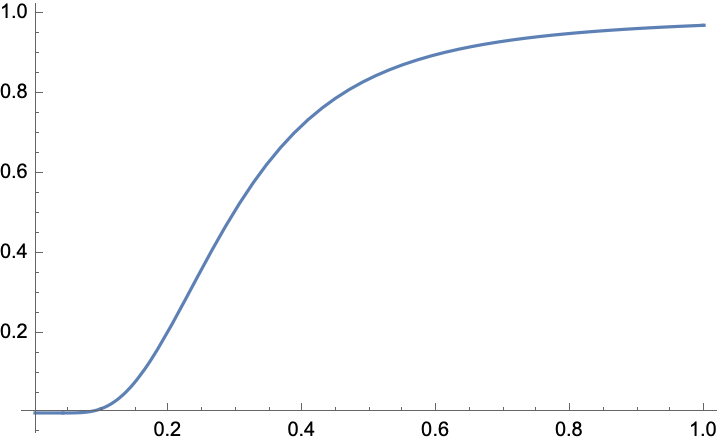
\includegraphics{q2d.png}
				\end{center}
				A bit of analysis: \( t = \frac{kT}{I}\), so increasing \( t \) is proportional 
				to increasing
				\( T \). Therefore, we can see that as temperature increases, a larger fraction of the 
				phosphorous atoms are ionized, which matches our intuition about what we intuitively 
				expect to happen at high temperatures. We also see that it becomes almost completely 
				ionized when \( I = kT \), which makes sense, since this corresponds to a situation where 
				almost all of the electrons in phosphorous are at or above the ionization energy.

				Also, the plot has a horizontal asymptote at 1 since we're plotting a ratio of ionized atoms.   
			\end{solution}
	\end{enumerate}
	\pagebreak
	\section*{Schroeder 5.83}
	Write down the equilibrium condition for each of the following reactions:
	\begin{enumerate}[label=\alph*)]
		\item \ch{2 H <-> H2}

			\begin{solution}
				As explained in the textbook, we just replace the \ch{<->} by an equality, 
				and replace the species by their chemical potentials. Therefore, this is:
				\[
					2\mu_H = \mu_{\ch{H_2}}
				\] 
			\end{solution}
		\item \ch{2 CO + O2 <-> 2 CO2}

			\begin{solution}
				Same thing:
				\[
					2\mu_{\ch{CO}} + \mu_{\ch{O_2}} = 2 \mu_{\ch{CO_2}}
				\] 
			\end{solution}
		\item \ch{CH4 + 2 O2 <-> 2 H2O + CO2}

			\begin{solution}
				And again..
				\[
					\mu_{\ch{CH_4}} + 2\ch{O_2} = 2\mu_{\ch{H_2O}} + \mu_{\ch{CO_2}}
				\] 
			\end{solution}
		\item \ch{H2SO4 <-> 2 H+ + SO4^2-}

			\begin{solution}
				Typing is hard\dots
				\[
					\mu_{\ch{H_2SO_4}} = 2\mu_{H^+} + \mu_{\ch{SO_4^2-}}
				\] 
			\end{solution}
		\item \ch{2 p + 2 n <-> ^4He}

			\begin{solution}
				Last one!
				\[
					2\mu_p + 2\mu_n = \mu_{\ch{He}}
				\] 
			\end{solution}
	\end{enumerate}
	\pagebreak
	\section*{Schroeder 5.84}
	A mixture of one part nitrogen and three parts hydrogen is heated, in the presence of a suitable catalyst, to
	a temperature of $500^\circ$ C. What fraction of the nitrogen (atom for atom) is converted to ammonia, if the 
	final total pressure is 400 atm? Pretend for simplicity that the gases behave ideally despite the very 
	high pressure. The equilibrium constant at $500^\circ C$ is \(6.9 \times 10^{-5}\). (Hint: You'll have to 
	solve a quadratic equation.)

	\begin{solution}
		The problem statement gives us that the final pressure is 400 atmospheres, so we know that 
		\[
			P_{\ch{H_2}} + P_{\ch{N_2}} + P_{\ch{NH_3}} = 400
		\] 
		Then, since we have 3 parts hydrogen for each 1 part nitrogen, then we also have:
		\[
			P_{\ch{H_2}} = 3P_{\ch{N_2}}
		\] 
		Finally, we use the law of mass action:
		\[
			K = \frac{P_{\ch{NH_3}}^2 (P^\circ)^2}{P_{\ch{N_2}} P_{\ch{H_2}}^3}
		\] 
		Then, since \( P^\circ \) is the background atmosphere (which is 1 in atmospheres), this then 
		simplifies to:
		\[
			P_{\ch{NH_3}} = \sqrt{27K} P_{\ch{H_2}}^2
		\] 
		Substituting this back into the first equation gives us our quadratic equation:
		\[
			4P_{\ch{N_2}} + \sqrt{27K} P_{\ch{N_2}}^2 = 400
		\] 
		Solving this quadratic using Mathematica, we get \( P_{\ch{N_2}} = 60.50 \), so we also 
		get \( P_{\ch{H_2}} = 181.505 \) and \( P_{\ch{NH_3}} = 157.994\). Finally, the ratio of the pressures
		gives a relationship between the fraction of reacted molecules, so we have to divide the partial pressure
		of ammonia with the partial pressure of nitrogen (we have to multiply the nitrogen by 2 since there are 
		2 particles in nitrogen):
		\[
			\frac{P_{\ch{NH_3}}}{2P_{\ch{N_2}}} = 1.31 \approx \frac{4}{3}
		\] 
		Therefore, the fraction of ammonia that gets converted is given by:
		\[
			\frac{N_{\ch{NH_3}}}{N_{\ch{NH_3} + N_{\ch{N_2}}}} = \frac{4}{4+3} = \frac{4}{7}
		\] 
		so we have \( \frac{4}{7} \) of the molecules are converted into ammonia.   
	\end{solution}
	\pagebreak
	\section*{Schroeder 5.85}
	Derive the \textbf{van't Hoff equation}, 
	\[
		\dv{\ln K}{T} = \frac{\Delta H^\circ}{RT^2}
	\] 
	which gives the dependence of the equilibrium constant on temperature. Here \(\Delta H^\circ\) is 
	the enthalpy change of the reaction, for pure substances in their standard states (1 bar pressure for 
	gases). Notice that if \(\Delta H^\circ\) is positive (loosely speaking, if the reaction requires the 
	absorption of heat), then higher temperature makes the reaction tend more to the right, as you 
	might expect. Often you can neglect the temperature dependence of \(\Delta H^\circ\) ; solve the equation 
	in this case to obtain
	\[
	\ln K(T_2) - \ln K(T_1) = \frac{\Delta H^\circ}{R}\left( \frac{1}{T_1} - \frac{1}{T_2} \right) 
	\] 

	\begin{solution}
		We have the equation that:
		\[
		e^{-\Delta G / RT} = K \implies \ln K = -\frac{\Delta G}{RT}
		\] 
		Therefore, now we can take the derivative:
		\[
			\pdv{\ln K}{T} = -\frac{1}{R} \pdv{\Delta G}{T}
		\] 
		We can then do this via quotient rule, since \( \Delta G \) is also a function of \( T \):
		\begin{align*}
			\pdv{\ln K}{T} &= -\frac{1}{RT^2}\left[ T\pdv{\Delta G}{T} - \Delta G \right] \\
			&= \frac{1}{RT^2}\left[ T(-\Delta S) - (\Delta H - T \Delta S) \right]  \\
			&= \frac{\Delta H}{RT^2} 
		\end{align*}
		In the first to second line, I've used the property that \( \pdv{\Delta G}{T} = -\Delta S \) from 
		the thermodynamic identities. For the second part of the problem, we basically just 
		have to solve a differential equation:
		\[
			d \ln K = \Delta \frac{H}{RT^2} dT
		\] 
		And now we can integrate both sides of this equation from \( T_1 \) to \( T_2 \). Note that 
		the problem tells us that \( \Delta H \) is independent of \( T \), so we can 
		pull it out of the integral:
		\begin{align*}
			\int_{T_1}^{T_2} d \ln K &= \frac{\Delta H}{R} \int_{T_1}^{T_2} \frac{1}{T^2} dT\\
			\left( \ln K \right)_{T_1}^{T_2} &= \frac{\Delta H}{R}\left(-\frac{1}{T}\right)_{T_1}^{T_2}
		\end{align*}
		Then, we can substitute the limits in, use logarithm rules to get:
		\[
		\ln K(T_2) - \ln K(T_1) = \frac{\Delta H}{R}\left( \frac{1}{T_1} - \frac{1}{T_2} \right) 
		\] 
		as desired.
	\end{solution}
\end{document}
